\graphicspath{{./stats/}}

\section{Results}
As described above, three independent variables (one of which was a repeated measures factor) and their interactions were analysed. These were assessed using nine dependant flow variables which can be aggregated into one higher-order factor. In order to analyse the results, a two-way repeated measures ANOVA was used for the higher-order factor, while a two-way repeated measures MANOVA was constructed with the results along the nine flow dimensions. The following sections describe the results of these analyses. Important findings are presented in bold.

\subsection{Higher-order flow factor analysis}
A two-way repeated measures ANOVA was conducted on the results of all three game genre groups. This ANOVA also considered the data from the three participant characteristics groups. The full results can be seen in Table~\ref{higherANOVA}. Mauchly's sphericity test was conducted to ensure normality within the data. The results of this test showed no deviations from the normality of variance assumptions required by ANOVA and so no correcting factors were used (\emph{p} =  0.360843).

\begin{table}

\centering %
\begin{tabular*}{0.75\textwidth}{@{\extracolsep{\fill}} l r r r r r }
	\hline	
	 Effect & SS & df & MS & F & \emph{p} \\
	\hline
	Intercept & 136549.2 & 1 & 136549.2 & 2934.263 & $<$ 0.000001* \\
	Genre & 4.6 & 2 & 2.3 & 0.050 & 0.951663 \\
	Group & 97.2 & 2 & 48.6 & 1.044 & 0.362406 \\
	Genre*Group & 327.8 & 4 & 82.0 & 1.761 & 0.158147 \\
	Error & 1675.3 & 36 & 46.5 & & \\
	\hline
	\hline
	Interface & 83.1 & 2 & 41.5 & 2.652 & 0.077416 \\
	Interface*Genre & 218.8 & 4 & 54.7 & 3.493 & 0.011565* \\
	Interface*Group & 45.8 & 4 & 11.4 & 0.731 & 0.573833 \\
	Interface*Genre*Group & 96.5 & 8 & 12.1 & 0.771 & 0.629683 \\
	Error & 1127.7 & 72 & 15.7   & & \\
	\hline
	\multicolumn{6}{l}{\emph{{\small * denotes a significant result at a 95\% confidence level ($\alpha$ = 0.05).}}} \\ 

	\end{tabular*}
\caption{Results of two-way (Genre-Participant characteristics) repeated measures (Interface) ANOVA conducted on the higher order flow factor results.}
\label {higherANOVA}
\end{table}

The only significant effect found was an interaction between \emph{Interface type} and \emph{Genre} (\emph{p} = 0.011565, $\alpha$ = 0.05). Tukey's HSD test was conducted on this interaction, but found no significant differences. A Fisher LSD test was then performed. The differences found are summarised in Table~\ref{lsdANOVA}. However, these results should be interpreted cautiously as this test has been criticised for not sufficiently controlling for Type I errors~\citep{Steve99}. Full results for both the Tukey HSD and Fisher LSD tests can be found in Appendix~\ref{appendix:higherOrder}. Figure~\ref{anova:cellMeans} plots the cell means with error bars for this interaction. By comparing cell means along with the results of the post-hoc testing, one can see that within the Strategy game genre, the direct manipulation interface version is preferred to the mixed version (\emph{M} = 33.8 and \emph{M} = 29.683, respectively). Within the Fighting/Duelling condition, the gestural version elicits more flow than the direct manipulation version (\emph{M} = 34.31 and \emph{M} = 30.3, respectively). The results of the other significant interactions will not be discussed further as they are across both game genre and interface type. Thus with regard to the higher-order factor, significant differences in the degree of flow experienced according to interface type were only present in the Strategy and Fighting/Duelling conditions.

\begin{table}

\centering %
\begin{tabular*}{0.9\textwidth}{@{\extracolsep{\fill}} c c | c c | r}
	\hline	 
	 \multicolumn{2}{c |}{Factor 1} & \multicolumn{2}{c |}{Factor 2} & \emph{p} \\
	 Genre & Interface type & Genre & Interface type & \\
	\hline
	Puzzle & Direct manipulation & Fighting/Duelling & Gestural & 0.029672* \\
	Strategy & Direct manipulation & Strategy & Mixed & 0.005719* \\
	Strategy & Mixed & Fighting/Duelling & Gestural & 0.014762* \\ 
	Fighting/Duelling & Direct manipulation & Fighting/Duelling & Gestural & 0.006940* \\
	\hline
	\multicolumn{5}{l}{\emph{{\small * denotes a significant result at a 95\% confidence level ($\alpha$ = 0.05).}}} \\ 

	\end{tabular*}
\caption{Summary of significant results of Fisher LSD conducted on the higher-order flow factor results.}
\label {lsdANOVA}
\end{table}

\begin{figure}[h]
  \begin{center}
    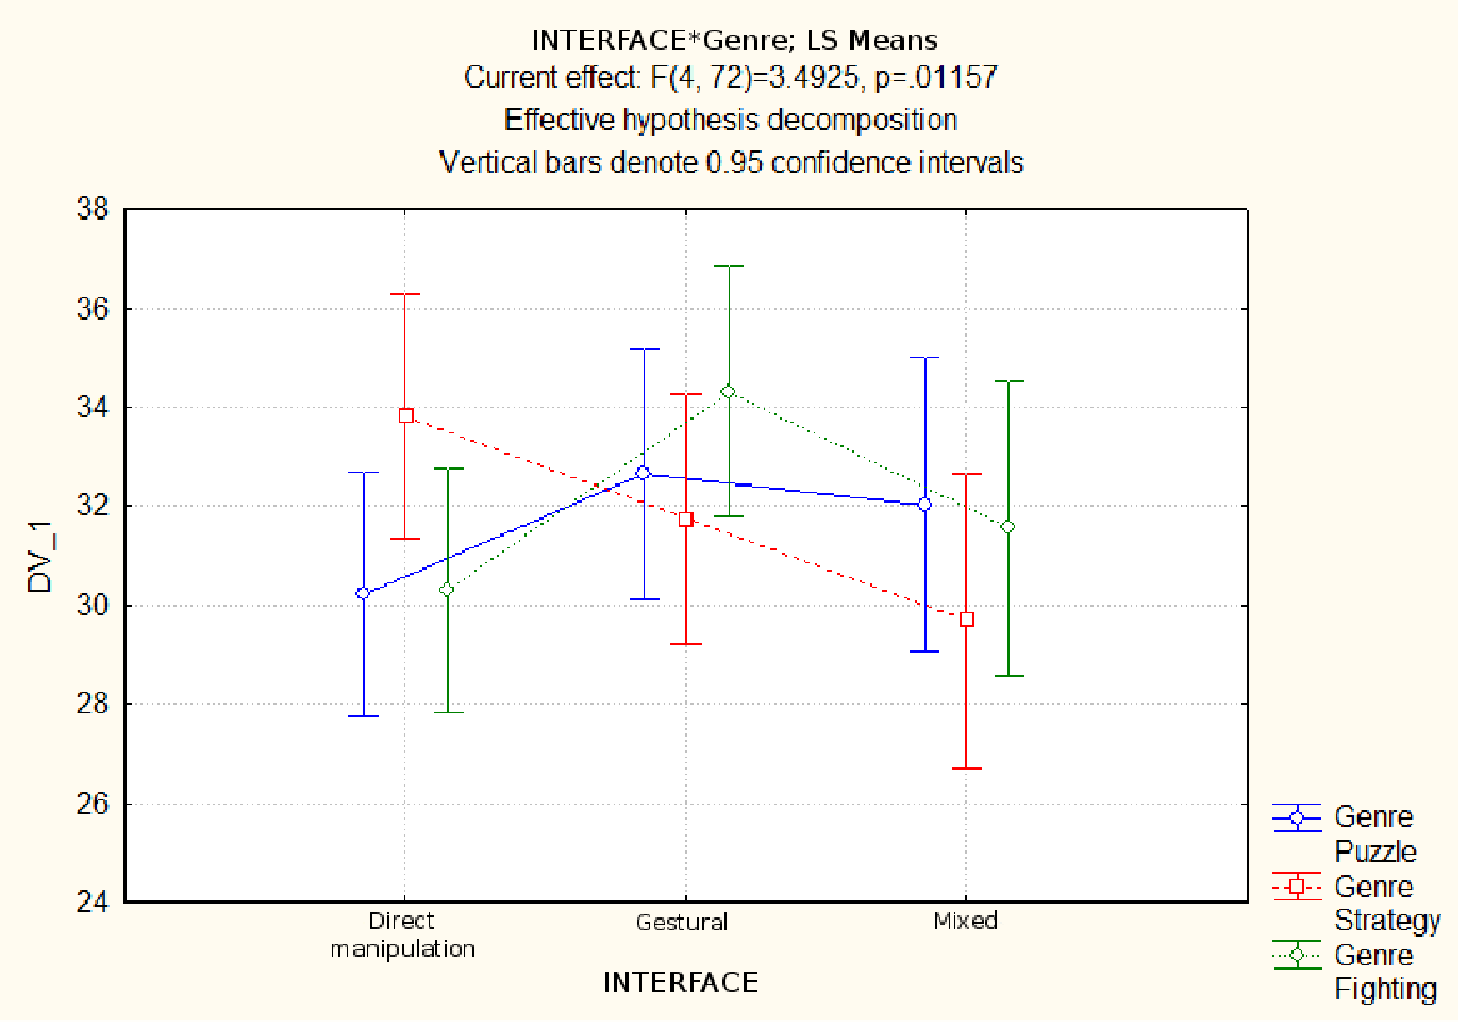
\includegraphics [scale=0.5]{anovaGraph.pdf}

  \end{center}
  \caption{Cell means plot for \emph{Genre}*\emph{Interface} interaction effect of higher-order flow factor ANOVA.}
  \label{anova:cellMeans}
\end{figure}

\subsection{Flow dimensions analysis}
The results across all nine flow dimensions were analysed using a two-way (Genre-Participant characteristic group) repeated measures (Interface) MANOVA with nine dependent variables. Mauchly's sphericity test was conducted to ensure normality. Full results for the test can be found in Appendix~\ref{manova:mauchly}. The assumption of normality was found to hold true for all dependent variables apart from \emph{Concentration on the task at hand} (\emph{p} = 0.035) and \emph{Transformation of time} (\emph{p} = 0.01). The Greenhouse-Geisser estimate was used to correct for this in the case of these two variables. 

The results of the MANOVA can be seen in Table~\ref{manova:all}. The reported \emph{p} values refer to the results obtained using Wilks' lambda distribution, which is a multivariate generalisation of the \emph{F}-distribution~\citep{Tred02}. An $\alpha$ value of 0.05 was used throughout. All main effects were found to be significant (Genre: \emph{p} = 0.006511; Group: \emph{p} = 0.043880; Interface: \emph{p} = 0.000005). In addition, the interaction between each pairwise combination of independent variables was also found to be significant (Genre*Group: \emph{p} = 0.006588; Interface*Group: \emph{p} = 0.025903; Interface*Genre: \emph{p} = 0.004767). However, the overall interaction between all three independent variables was not found to be significant (\emph{p} = 0.644534).

\begin{table}

\centering %
\begin{tabular*}{0.8\textwidth}{@{\extracolsep{\fill}} l r r r r r }
	\hline	
	 Effect & Value & F & Effect df & Error df & \emph{p} \\
	\hline
	Intercept &  0.009898 & 311.2176 & 9 & 28.0000 & $<$ 0.000001* \\
	Genre &  0.318534 & 2.4013 & 18 & 56.0000 & 0.006511* \\
	Group & 0.396239 & 1.8313 & 18 & 56.0000 & 0.043880* \\
	Genre*Group &  0.157573 & 1.8885 & 36 & 106.6663 & 0.006588* \\
	Interface & 0.099285 & 9.5760 & 18 & 19.0000 & 0.000005* \\
	Interface*Genre &  0.094389 & 2.3802 & 36 & 38.0000 & 0.004767* \\
	Interface*Group &  0.126765 & 1.9091 & 36 & 38.0000 & 0.025903* \\
	Interface*Genre*Group &  0.087785 & 0.9168 & 72 & 77.0695 & 0.644534 \\
	\hline
	\multicolumn{6}{l}{\emph{{\small * denotes a significant result at a 95\% confidence level ($\alpha$ = 0.05).}}} \\ 

	\end{tabular*}
\caption{Results of two-way (Genre-Participant characteristics) repeated measures (Interface) MANOVA conducted on the nine flow dimensions. Wilks' lambda distribution test is used.}
\label {manova:all}
\end{table}

In order to better understand the nature of these interactions, post-hoc testing was conducted for each significant interaction along all dependent variables. A summary of these flow factors and their meaning can be found in Table~\ref{flowDimen}. In addition, univariate repeated measures tests for each dependent variable were conducted. The full results of all these tests are contained in Appendix~\ref{manova:univar} and Table~\ref{manova:summary} contains a summary of our findings. The following sections will describe the results of these tests according to these interactions and main effects.

\begin{table}[!h]
\footnotesize
\centering %
\begin{tabular*}{\textwidth}{@{\extracolsep{\fill}} p{3cm} | l l l r | c | l l l r | r}
	\hline	
	Factor & \multicolumn{4}{c |}{Condition 1} & & \multicolumn{4}{c |}{Condition 2} \\
	& Interface & Genre & Group & \emph{M} &  & Interface & Genre & Group & \emph{M} & \emph{p} \\
	\hline
	\multirow{7}{3cm}{Challenge-Skill Balance} & DM & & & 11.622 & $<$ & G & & & 15.289 & 0.000111* \\
	& DM & & &11.622& $<$ & M& & & 14.933 & 0.000111* \\
	& DM & P & & 9.333 & $<$ & G & P & & 14.067 & 0.000293* \\
	& DM & P & & 9.333 & $<$ & M & P & & 13.200 & 0.004324* \\
	& DM & F & & 12.400 & $<$ & G & F & & 15.600 & 0.000152* \\
	& DM & F & & 12.400 & $<$ & M & F & & 15.733 & 0.000145* \\
	& DM & & G & 11.467 & $<$ & G & & G & 15.667 & 0.001410* \\
	& DM & & T & 12.067 & $<$ & G & & T & 16.400 & 0.000908* \\
	& DM & & T & 12.067 & $<$ & M & & T & 16.667 & 0.000405* \\
	\hline
	\multirow{2}{3cm}{Merging of Action and Awareness} & DM & & & 13.667 & $<$ & G& & & 15.622 & 0.001201* \\
	& DM & & & 13.667& $<$ & M & & & 15.511 &  0.002278* \\
	\hline
	\multirow{6}{3cm}{Clear Goals} & DM & & & 12.578 & $<$ & G & & & 15.356 & 0.000114* \\
	& DM & & &  12.578& $<$ & M & & & 15.200 &  0.000121* \\
	& DM & F & & 12.467 & $<$ & G & F & & 16.400 & 0.001737* \\
	& DM & F & & 12.467 & $<$ & M & F & & 16.267 & 0.002781* \\
	& DM & & G & 12.000 & $<$ & G & & G & 15.667 & 0.000855* \\
	& DM & & G & 11.533 & $<$ & M & & G & 15.200 & 0.004454* \\
	\hline
	\multirow{2}{3cm}{Unambiguous Feedback} & DM & F & & 10.867 & $<$ & G & F & & 15.267 & 0.000921* \\
	& & & & & & & & & & \\
	\hline
	\multirow{2}{3cm}{Concentration on the Task at Hand} & DM & & & 13.267& $<$& G & & & 15.511 & 0.005088* \\
	& & & & & & & & & & \\
	\hline
	\multirow{4}{3cm}{Sense of Control} & DM  & & &  12.467&$<$ &G & & &  14.889 & 0.000209* \\
	& M & & & 13.356& $<$ &G & & & 14.889 &  0.018505* \\
	& DM & & G & 11.533 & $<$ & G & & G & 15.133 & 0.039190* \\
	& DM & & T & 11.800 & $<$ & G & & T & 15.600 & 0.004790* \\
	\hline
	\multirow{2}{3cm}{Loss of Self-Consciousness} & M & S & & 10.333 & $<$ & G & S & & 14.600 & 0.016831* \\
	& M & S & & 10.333 & $<$ & DM & S & & 16.333 & 0.000233* \\
	\hline
	\multirow{2}{3cm}{Transformation of Time} &  M & & & 13.156& $<$& DM & & & 15.556 &  0.001579* \\
	& M & S & & 11.133 & $<$ & DM & S & & 15.067 & 0.025650* \\
	\hline
	\multirow{4}{3cm}{Autotelic Experience} & G & & & 12.444& $<$ &DM & & & 14.778 & 0.003083* \\
	& M & & & 12.156& $<$ &DM & & & 14.778 &  0.000863* \\
	& M & S & & 9.333 & $<$ & DM & S & & 13.933 & 0.006637* \\
	& G & & G & 10.667 & $<$ & DM & & G & 14.667 & 0.030455* \\
	\hline
	\multicolumn{11}{l}{\emph{Key:}} \\
	\multicolumn{11}{l}{\emph{Interface: DM - Direct manipulation, G - Gestural, M - Mixed}} \\
	\multicolumn{11}{l}{\emph{Genre: P - Puzzle, S - Strategy, F - Fighting/Duelling}} \\
	\multicolumn{11}{l}{\emph{Group: G - Gaming experience, T - Touch-device experience, C - Control}} \\
	\hline
	\multicolumn{11}{l}{\emph{{\small * denotes a significant result at a 95\% confidence level ($\alpha$ = 0.05).}}} \\ 

	\end{tabular*}
\caption{Summary of all Tukey HSD post-hoc testing and univariate results decomposed according to \emph{Interface}, \emph{Genre} and \emph{Group}. Only meaningful significant results are included above. Condition 1 and 2 refer to the two combinations of \emph{Interface}, \emph{Genre} or \emph{Group} that produced a significant difference. Blank column entries for a row mean this factor is not included in the combination. The inequality indicates the nature of the significant result, as can be seen by comparing their means.}
\label {manova:summary}
\end{table}

\subsubsection{\emph{Interface}*\emph{Genre}}
Tukey's HSD test was conducted on this interaction for each dependent variable. In addition, univariate testing showed this interaction as significant for the \emph{Unambiguous Feedback} and \emph{Loss of Self-Consciousness} dimensions. The results discussed below refer to the findings of these tests. In the discussion only those results with some meaningful interpretation are mentioned. That is, significant differences between both different interface types and genres are not elaborated on.

A significant effect was shown between the direct manipulation version of the Puzzle game and all other game combinations except the Fighting/Duelling direct manipulation interface along the \emph{Challenge-Skill Balance} dimension. In all cases, the mean for the direct manipulation Puzzle game was lower than the other combinations. This suggests that this condition elicited the lowest degree of flow along this dimension. In addition, the same was true of the direct manipulation Fighting/Duelling version when compared to the Fighting/Duelling gestural and mixed interfaces (Gestural: \emph{p} = 0.035257; Mixed: \emph{p} = 0.023826). No meaningful significant results were obtained for the \emph{Merging of Action and Awareness} dimension.

With regard to the results of post-hoc testing along the \emph{Clear Goals} dimension, the only significant result of note is the lower score of direct manipulation in the Fighting/Duelling condition when compared to this genre's other two interface types (Gestural: \emph{p} = 0.001737; Mixed: \emph{p} = 0.002781). \emph{Unambiguous Feedback} showed a significant interaction between \emph{Interface} and \emph{Genre} in the univariate testing. Post-hoc testing was also conducted for this variable. The only meaningful significant results was a difference between the Fighting/Duelling direct manipulation and gestural versions (\emph{p} =  0.000921). A cell mean plot indicated that the gestural version elicited more flow along this dimension than the direct manipulation version.

Post-hoc testing did not reveal any significant results for either \emph{Concentration on the Task at Hand} or \emph{Sense of Control} for this interaction. \emph{Loss of Self-Consciousness} showed significant results in both Tukey's HSD and the univariate testing. The mixed interface version of the Strategy game was shown to produce less \emph{Loss of Self-Consciousness} than either of the other two interface versions (Gestural: \emph{p} = 0.016831; Direct manipulation: \emph{p} = 0.000233). The \emph{Transformation of Time} and \emph{Autotelic Experience} dimensions showed a significant difference between the Strategy direct manipulation and mixed versions. For both variables, the direct manipulation interface elicited more flow than the mixed one.

When examining the cell means plots of the interaction across the nine dependent variables, in general, all interactions are ordinal. That is, they have simple effects that lie in the same direction~\citep{Tred02}. This ordinal interaction holds true more so for the Strategy and Fighting/Duelling games than for the Puzzle and either of the other two. Overall, when considering these graphs, the majority of disagreement between genres seems to lie with the mixed interface. When disregarding this condition, the disordinal effects are only introduced by the Strategy game. Thus it appears that there is more overall agreement on interface preference between the Strategy and Fighting/Duelling games, but that disordinal interactions are present between Strategy and the other two genres when considering only the direct manipulation and gestural versions. Most importantly, no significant differences were found between the same interface type and two or more different \emph{Genres} across any of the variables. {\bf In addition, the nearly parallel nature of the mean plots for each genre across a number of dimensions, suggests that while some interface version may be significantly preferred within a single genre, there are no significant overall inter-genre difference with regard to interface preference.}


\subsubsection{\emph{Interface}*\emph{Group}}
No significant univariate results were found for this interaction. Tukey's HSD test, however, revealed a number of significant effects between conditions of this interaction. In general, no significant or meaningful results were found for \emph{Merging of Action and Awareness}, \emph{Unambiguous Feedback}, \emph{Concentration on the Task at Hand}, \emph{Loss of Self-Consciousness} or \emph{Transformation of Time}. Once again, only the meaningful differences are discussed below.

\emph{Challenge-Skill Balance} showed a significant difference between the Gaming experience direct manipulation and gestural versions (\emph{p} = 0.001410). Significant differences were also found within the Touch-device experience group between the direct manipulation interface and both of the other versions (Gestural: \emph{p} = 0.000908; Mixed: 0.000405). In all three cases, the direct manipulation interface elicited less flow along this dimension than the other interfaces. Post-hoc testing on the \emph{Clear Goals} variable showed the direct manipulation interface produced significantly less flow than either of the other two versions (Gestural: \emph{p} = 0.000855; Mixed: \emph{p} = 0.004454). The direct manipulation version was also shown to elicit significantly less flow along the \emph{Sense of Control} dimension than the gestural version for both the Gaming and Touch-device experience groups (\emph{p} = 0.039190 and \emph{p} = 0.004790, respectively). Finally, in the \emph{Autotelic Experience} condition, the gestural interface produced less flow than the direct manipulation version (\emph{p} = 0.030455).

Ordinal interactions between the Control and Touch-device experience groups were present along all dimensions, except \emph{Sense of Control}. In addition, in many of the cell mean plots, the interaction between the Control and Touch-device experience groups is almost parallel between some or all of the interface versions. This, along with the results of the post-hoc testing suggest that there may be very little difference between these groups. The same was not true between Gaming experience and either of the other two groups, where a disordinal interaction between one or both of the other groups was present along every dimension. This suggests some difference between how flow is experienced within the Gaming experience group and the other two groups. The post-hoc testing supports this to some degree, showing significant differences between the Gaming experience conditions and those of the Touch-device experience and Control groups. However, none of these differences lie across the same interface version. Multivariate contrast analysis was used to asses this further. This showed a significant difference between the Gaming experience and Control groups (\emph{p} = 0.014123). When comparing means for these two groups both on a variable by variable basis, as well as overall, the Gaming experience group appears to experience more flow than the Control group. While no significant difference was found between Gaming and Touch-device experience, a significant difference was present between the Control and Touch-device experience groups (\emph{p} = 0.035751). When comparing per-variable means, the Touch-device experience group seems to experience more flow along all dimensions except \emph{Concentration on the Task at Hand} and \emph{Sense of Control}. The overall means also suggest that more flow is elicited in those with touch-device experience than without. {\bf This suggests that both gaming and previous touch-device experience increase the degree to which a flow state is experienced.}

\subsubsection{\emph{Interface} main effect}
Univariate testing revealed a significant \emph{Interface} main effect for all dependent variables. In addition, a significant interaction between \emph{Interface type} and \emph{Genre} was found for \emph{Unambiguous Feedback} and \emph{Loss of Self-Consciousness}. For this reason, the main effect in these two cases will not be investigated further. Tukey's HSD was performed on the \emph{Interface} main effect for all other dependent measures.

Significant differences were found between the direct manipulation interface and both the gestural and mixed interfaces for \emph{Challenge-Skill Balance} (\emph{p} = 0.000111 in both cases), \emph{Merging of Action and Awareness} (Gestural: \emph{p} = 0.001201; Mixed: \emph{p} = 0.002278), \emph{Clear Goals} (Gestural: \emph{p} = 0.000114; Mixed: \emph{p} = 0.000121) and \emph{Autotelic Experience} (Gestural: \emph{p} = 0.003083; Mixed: \emph{p} = 0.000863). In the case of the first three variables, the cell means plots indicate that the direct manipulation version elicited less flow along these dimensions than either the gestural or mixed interface versions. The direct manipulation interface elicited more flow along the \emph{Autotelic Experience} dimension than the other two interface types, however. 

The \emph{Concentration on the Task at Hand} dimension was shown to produce a higher flow effect in the gestural interface when compared to the direct manipulation interface (\emph{p} = 0.005088). In the case of \emph{Sense of Control}, the gestural interface was shown to elicit this dimension more highly than either of the other two interfaces (Direct manipulation: \emph{p} = 0.000209; Mixed: \emph{p} = 0.018505). Finally, the direct manipulation interface elicited more flow along the \emph{Transformation of Time} dimension than the mixed interface (\emph{p} = 0.001579).

Multivariate contrast analysis was used to attempt to collapse these results across all dependent variables. This provided significant results for all possible interface pairwise combinations (Direct manipulation - Gestural: \emph{p} = 0.000002; Direct manipulation - Mixed: \emph{p} = 0.000012; Gestural - Mixed: \emph{p} = 0.033951). {\bf Overall means for these three conditions show that more flow is elicited in the gestural condition than in either of the other two and that the mixed interface produces more flow than the direct manipulation interface.}

\subsection{Puzzle game results}
Multivariate contrast analysis was used to determine the effects of \emph{Interface} and \emph{Group} within the Puzzle game genre. This was chosen instead of a separate MANOVA as there would then be more dependent variables than subjects in each of the subject participant groups which would decrease both the power and validity of the analysis. 

The results of the contrast analysis for \emph{Interface} show significant differences between the gestural version and both the direct manipulation and mixed interfaces (Direct manipulation: \emph{p} = 0.000031; Mixed: \emph{p} = 0.014434). When examining the overall means for these conditions, they show that the gestural version elicits more flow than either the direct manipulation or mixed versions. The interaction between \emph{Interface} and \emph{Group} was also subjected to Multivariate contrast analysis. The only significant effect was found between the Gaming and Control conditions (\emph{p} = 0.008096). Cell means for these two conditions suggest that those with significant gaming experience more readily experience flow than those with limited gaming experience. 

{\bf Both of these contrast analyses provide findings that correspond with those found across all three genres.} However, the lack of any difference between the mixed and direct manipulation interfaces, as well as between Touch-experience and Control groups, may suggest that these differences are introduced by the other genres.
